\documentclass[10pt]{article}
\usepackage[a4paper,margin=20mm]{geometry}
\usepackage{booktabs,graphicx}
\graphicspath{{../../experiments/results/}}
\title{Software AES vs.\ Zkne vs.\ AES Engine for Model Protection on RISC-V}
\author{Gaurav, IIIT Hyderabad}
\date{November 2026}
\begin{document}
\maketitle

\paragraph{Question.} Neural-network weights must be decrypted (AES-128-CTR) and authenticated (AES-CMAC) before an
accelerator uses them. What does each of three ways cost in time, CPU and area:
software AES on the CVA6 host, (A) Zkne AES instructions in CVA6, or (B) OpenTitan AES with a DMA on the system bus?

\paragraph{Setup.} Upstream CVA6 (RV64GC + Zkn) in its VCS test harness; Option B added as AXI masters
(unmasked and masked OpenTitan AES, our DMA with an AES streaming mode). Int8 MNIST models of 12\,KB, 102\,KB and 1.07\,MB
(97.8--98.5\,\% accuracy), 4\,KB tiles, tag per tile. Area: Genus, TSMC 65\,nm LP, 4\,ns clock, logic only.
All 24 runs decrypt correctly, reject a flipped bit, and reproduce the reference inference outputs.

\begin{table}[h]\centering\small
\begin{tabular}{lrrrr}\toprule
Method & Check+decrypt (cyc/B) & vs.\ software & CPU busy (cyc/B) & Area (kGE)\\\midrule
Software AES & 141 & $1\times$ & 141 & 0\\
A: Zkne & 9.6 & $14.7\times$ & 9.6 & 5.9\\
B: engine, unmasked & 2.7 & $52.6\times$ & 0.40 & 51.7\\
B: engine, masked & 7.5 & $18.8\times$ & 0.44 & 106.1\\\bottomrule
\end{tabular}
\caption{4\,KB tiles; speed-ups are for the 102\,KB and 1.07\,MB models, which give the same cycles/byte.
Zkne area is the Zkn unit alone (1.6\,\% of CVA6's 374\,kGE). Engine area includes the 13.8\,kGE DMA.}
\end{table}

\paragraph{Findings.}
\begin{itemize}\itemsep0pt
\item Software AES is too slow to be practical: 141 cycles/byte, all of it on the CPU.
\item Zkne gives a $14.7\times$ speed-up over software for 5.9\,kGE, but still uses the whole core while it runs.
\item The engine is fastest: $3.6\times$ (unmasked) / $1.3\times$ (masked) faster than Zkne once tiles exceed 130\,B / 470\,B,
  and it frees the CPU (0.4 vs.\ 9.6 busy cycles/byte).
\item Zkne costs $9\times$ less area than the unmasked engine and gives $2\times$ its throughput per kGE ($12\times$ that of the masked engine).
\item Small tiles hurt the engine more than Zkne (1\,KB vs.\ 64\,KB tiles: 3.96 vs.\ 2.28 cyc/B for the engine, 10.2 vs.\ 9.4 for Zkne),
  because each tile costs about 1{,}750 cycles of engine set-up.
\item Zkne does not limit Fmax: CVA6 meets 400\,MHz with and without it.
\end{itemize}

\begin{figure}[h]\centering
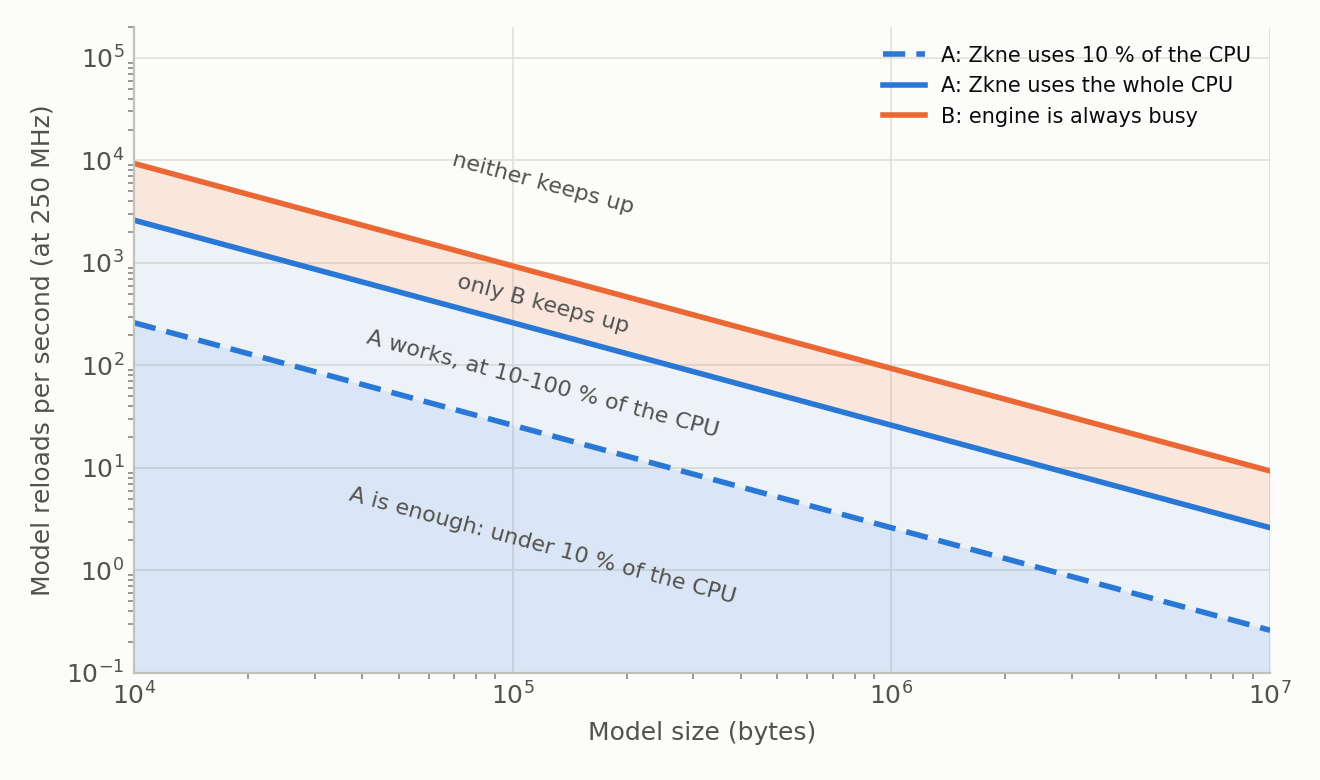
\includegraphics[width=0.75\linewidth]{break_even.png}
\caption{Which option keeps up, by model size and reload rate (250\,MHz).}
\end{figure}

\paragraph{Conclusion.} Software AES is only an option when area is fixed and models are loaded rarely.
Zkne is the cheap choice for small or rarely reloaded models (under $\sim$2.7\,MB/s at 10\,\% CPU);
a dedicated engine is needed for large or frequently reloaded models, or when the CPU must stay free.

\paragraph{Limits.} No PULP cluster or HyperRAM (DMA copies stand in); Zkne is unmasked; whole-core area varies by 1--2\,kGE between runs.
\end{document}
